\chapter{Project Organization and Structure} 
% Main chapter title

\label{Chapter4} 
%Call reference to this chapter use \ref{ChapterX}

\lhead{Chapter 4. \emph{Project Organization and Structure}} 
% Change X to a consecutive number; this is for the header on each page - perhaps a shortened title

\doublespacing
% LINE FORMATTING

%\clearpage
%\pagebreak

% MAIN SECTION ==============================
\section{Manpower}
This project is handled by four Software engineering students. That leads everyone to handle more than one position which produce a higher quality product after each prototype.
\pagebreak
\section{Project Organization and Structure}
Team members are having a role rotation plan that designed to enhance the product by team members abilities. Below is the organization chart shows basic roles:
\begin{figure}[H]
	\centering
	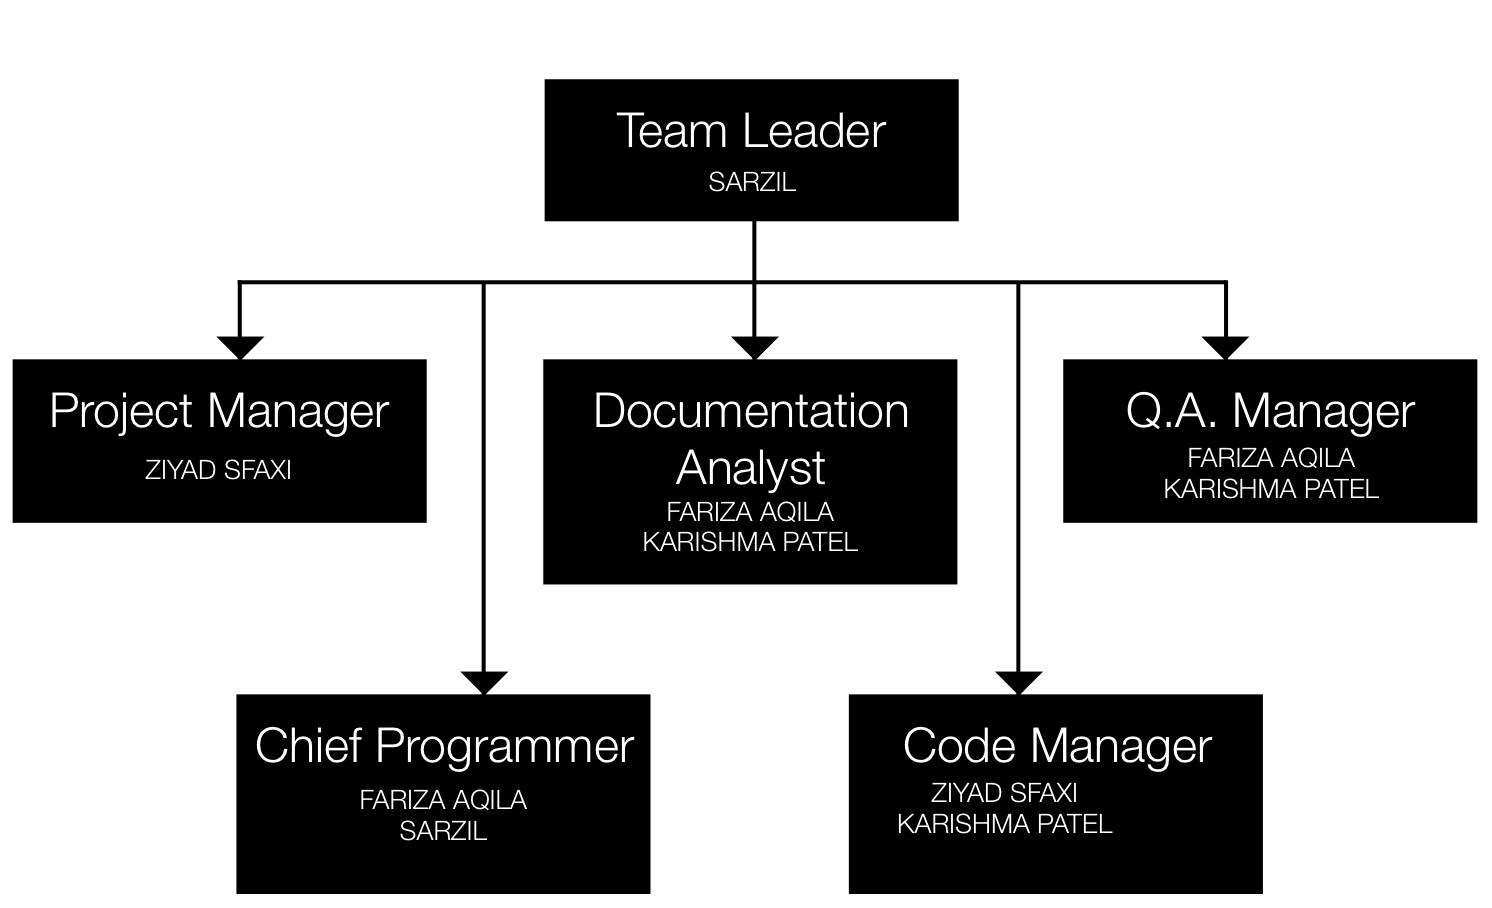
\includegraphics[scale=0.5]{Figures/FigureOrganizationChart.png}
	\rule{35em}{0.5pt}
	\caption[Organization Chart]{Organization Chart}
\end{figure}
\pagebreak

Below is a table that descripe every role:

\begin{table}[H]
	\centering
	\begin{tabular}{|p{4cm}|p{9.5cm}|}
		\hline
		{\bf ORGANIZATION}             & \bf DESCRIPTION                              \\ \hline
		{\bf Team Leader}           &  \begin{itemize}
			\item Serve as main contact with the managers.
			\item Ensuring the team is consistently delivering working software to the standards the department expects.
			\item Ensuring the team is self-organising so that we take collective responsibility for the work we do.
		\end{itemize}\\ \hline
		{\bf Project Manager} & \begin{itemize}
			\item Rotate roles to maximize the result of team abilities.
			\item Coordinate all those resources and the team’s tasks – to make sure that work is done in the proper sequence with a minimum of time.
			\item Ensuring the scope project is delivered and the body of  work is accomplished.
		\end{itemize}\\ \hline
		 \end{tabular}\end{table}
	\pagebreak \clearpage
	\begin{table}[H]
	\begin{tabular}{|p{4cm}|p{9.5cm}|}
		\hline
		{\bf Q.A. Manager}           &  \begin{itemize}
			\item Assures the viability, functionality and effectioness of essential tools.
			\item Anticipates program release problems and takes coorective action, escalation as needed, to resolve and achieve commitments.
		\end{itemize}\\ \hline
		{\bf Documentation
			Analyst}& \begin{itemize}
			\item Ensure that all documents have no errors in filenames or submissions.
			\item Perform evaluations and document audits.
		\end{itemize}\\ \hline
		
		{\bf Chief Programmer}  &  Convert the design and to a programming langauge.\\ \hline
		{\bf Code Manager} & Maintain the record of code files and the make file(s)\\ \hline

	\end{tabular}
	\caption{Table of organization roles}
	\label{Table of organization roles}
\end{table}
